%=========================================================================
% (c) Michal Bidlo, Bohuslav Křena, 2008

% tikzit regex: (,)?\s*style=\w*(,)?\s*

% \listoftodos

\chapter{Introduction}
Nowadays, when malicious code or malware is becoming more and more sophisticated and pressing security risk, it is really needed to control a program behaviour and monitor what the program is doing in a system.
Monitoring program behaviour can be done in many ways and one of the easiest ways is to use Intrusion Detection System (IDS).
IDS is an out-of-the-box solution which can monitor i.e. where program wrote or read something and it is not allowed.
After that, IDS is reporting this violation.

Another way is to monitor and block system calls (syscalls).
Monitoring is performed using tools mentioned in the next chapter.
The actual blocking can be performed with mandatory control access (MAC) (Apparmor, SELinux), sandboxing (seccomp) or others mechanisms.
MAC refers to a type of access control by which the operating system constraints the ability of a subject or initiator to access or generally perform some sort of operation on an object or target.
Seccomp is a Linux kernel module which allows a process one-way transition to secure a state where the process can only use four syscalls.
When the process tries to call another syscall then one of the four member's sets is terminated with SIGKILL.
The set of allowed system calls can be extended using seccomp-bpf.
This extension allows filtering system calls using a configurable policy implemented with Berkley Packet Filter (BPF) rules.
This last part is an area on which I would like to focus in my thesis.

I aim to design and develop a tool which helps developers using libseccomp and seccomp-bpf.
I plan to create policies for a specific program in a format readable by libseccomp or seccomp-bpf.

\Cref{chap:syscalls} describes syscalls and how to monitor them.
In the next chapter of the thesis, I will illustrate how security facilities in Linux, such as systrace and seccomp, work.
After the theoretical part, the design and development of a tool will follow.
In conclusion, methodology how this tool was tested is described.

\chapter{System Calls and Monitoring Tools}
\label{chap:syscalls}
In this chapter, I will describe a term system call and make an overview of tools which can monitor the system calls.
We will focus in detail on a strace tool which will be used as an input to my tool.
The other applications are described briefly not as detailed as the strace tool.

\section{System Calls}

In computer terminology, the term syscall is a way in which a computer program requests a service of the operating system on which is executed on.
In other words, the system calls are functions used in the kernel itself.
The system call appears to a standard developer as a C function call.
This design is typical for monolithic kernels.
We can find them on every UNIX system.
The system calls are generated using interruption, i.e., on Linux/i86 with an interruption no. \texttt{0x80} or with a system call named \texttt{syscall()} or \texttt{sysenter()} and these syscalls are handled by the kernel in a privileged mode.
When a user invokes a system call, an execution flow is as follows:
\begin{itemize}
	\item Each syscall is vectored through a stub in libc.
    	  Some syscalls are more complicated than others because of a variable length of the arguments, but the entry point and the end point of syscall are still the same.
	\item In libc, the number of the syscall is then set to an \texttt{eax} register, and the stack frame is also set up.
	\item An interrupt number \texttt{0x80} is called and transferred to the kernel entry point.
    	  The entry point is the same for every system call.
	\item In the table of interrupts, a pointer to interruption handler is found.
    	  After that, the execution of the interrupt handler follows which stores the content of the CPU registers and checks if a valid syscall is called.
	\item The handler finds the corresponding offset in the table of interrupts \texttt{\_sys\_call\_table}, where a pointer to the syscall service is stored.
	\item Control is transferred to the syscall service.
	\item Syscall returns a value to the register \texttt{EAX} on a 32-bit architecture or \texttt{RAX} on a 64-bit architecture.
	\item At the end of the syscall, \texttt{\_ret\_from\_sys\_call\(\)} is called.
    	  This call is done before returning to userspace.
          It checks if the scheduler should be run, and if so, it calls it.
	\item Immediately after return from the system call to interrupt handler, \texttt{syscallX()} macro checks for a negative return value from the syscall, if so it puts a positive copy of a return value to a global variable \texttt{\_errno}, for accessing from code like \texttt{perror()}.
\end{itemize}

This procedure is illustrated in Figure \ref{fig:tikz:int_handling}.

\begin{figure}[]
  \centering
  % \includestandalone[]{obrazky-figures/mytikz}%     without .tex extension
  \begin{tikzpicture}[align=left, thick]
	\begin{pgfonlayer}{nodelayer}
		\node [] (0) at (-5, 5) {};
		\node [] (1) at (-4, 5) {};
		\node [] (2) at (-5, 3.75) {};
		\node [] (3) at (-4, 3.75) {};
		\node [] (4) at (-2, 6) {};
		\node [] (5) at (-2, 3.25) {};
		\node [] (6) at (1, 3.25) {};
		\node [] (7) at (1, 6) {};
		\node [] (8) at (-4, 4.5) {};
		\node [] (9) at (-4, 4.25) {};
		\node [] (10) at (-2, 4.5) {};
		\node [] (11) at (-2, 4.25) {};
		\node [] (12) at (-5, 4.5) {};
		\node [] (13) at (-6, 4.5) {};
		\node [] (14) at (-6, 2) {};
		\node [] (15) at (-8, 2) {};
		\node [] (16) at (2.25, 2) {};
		\node [] (17) at (-6, 1) {};
		\node [] (18) at (-8, 1) {};
		\node [] (19) at (-6.25, 1) {};
		\node [] (20) at (-5.75, 1) {};
		\node [] (21) at (-4.25, 1) {};
		\node [] (22) at (-4.25, -0) {};
		\node [] (23) at (-5.75, -0) {};
		\node [] (24) at (-6, -0) {};
		\node [] (25) at (-6.25, -0) {};
		\node [] (26) at (-8, -0) {};
		\node [] (27) at (-6, 0.5) {};
		\node [] (28) at (-4.5, -0.75) {};
		\node [] (29) at (-4.5, -1.75) {};
		\node [] (30) at (-3.5, -1.75) {};
		\node [] (31) at (-3.5, -0.75) {};
		\node [] (32) at (-4, -1.25) {};
		\node [] (33) at (-4.5, -1.25) {};
		\node [] (34) at (-2, -0) {};
		\node [] (35) at (-2, -2.5) {};
		\node [] (36) at (-1, -2.5) {};
		\node [] (37) at (-1, -0) {};
		\node [] (38) at (-2, -0.75) {};
		\node [] (39) at (-1, -0.75) {};
		\node [] (40) at (-1, -1.25) {};
		\node [] (41) at (-2, -1.25) {};
		\node [] (42) at (0, -0) {};
		\node [] (43) at (1, -0) {};
		\node [] (44) at (1, -1) {};
		\node [] (45) at (0, -1) {};
		\node [] (46) at (0, -1.75) {};
		\node [] (47) at (1, -1.75) {};
		\node [] (48) at (1, -2.75) {};
		\node [] (49) at (0, -2.75) {};
		\node [] (50) at (-1.5, -1) {};
		\node [] (51) at (0, -0.5) {};
		\node [] (52) at (-2, -1) {};
		\node [] (53) at (-3.75, -0.5) {};
		\node [] (54) at (0.5, -0) {};
		\node [] (55) at (-4, -0.5) {};
		\node [] (56) at (-4.25, 3.5) {};
		\node [font={\tiny}, right, align=left,] (57) at (-7.75, 2.25) {User space};
		\node [font={\tiny}, right, align=left,] (58) at (-7.75, 1.75) {Kernel space};
		\node [align=left, rotate=270, font=\small] (59) at (-5.75, 3) {\texttt{int \$0x80}};
		\node [] (60) at (-4.5, 5.25) {libc};
		\node [] (61) at (-0.5, 6.25) {source.c};
		\node [font={\small}, align=left,] (62) at (-0.75, 5.5) {int main()\{};
		\node [font={\small}, align=left,] (63) at (-0.25, 5) {printf("42")\;};
		\node [font={\small}, align=left,] (64) at (-0.5, 4.5) {return 0;};
		\node [font={\small}, align=left,] (65) at (-1.5, 4) {\}};
		\node [] (66) at (-4, -2.25) {};
	\end{pgfonlayer}
	\begin{pgfonlayer}{edgelayer}
		\draw [] (0.center) to (1.center);
		\draw [] (0.center) to (2.center);
		\draw [] (2.center) to (3.center);
		\draw [] (3.center) to (9.center);
		\draw [] (9.center) to (8.center);
		\draw [] (8.center) to (1.center);
		\draw [->, thick] (8.center) to (10.center);
		\draw [<-, loosely dashed, thick, in=180, out=0, looseness=1.00] (9.center) to (11.center);
		\draw [] (11.center) to (10.center);
		\draw [] (4.center) to (10.center);
		\draw [] (5.center) to (11.center);
		\draw [] (5.center) to (6.center);
		\draw [] (6.center) to (7.center);
		\draw [] (7.center) to (4.center);
		\draw [thick,] (12.center) to (13.center);
		\draw [thick,] (13.center) to (14.center);
		\draw [ultra thick,] (14.center) to (15.center);
		\draw [, ultra thick] (14.center) to (16.center);
		\draw [thick, ->] (14.center) to (17.center);
		\draw [] (17.center) to (20.center);
		\draw [] (20.center) to (21.center);
		\draw [] (22.center) to (23.center);
		\draw [] (20.center) to (23.center);
		\draw [] (23.center) to (24.center);
		\draw [] (24.center) to (25.center);
		\draw [] (25.center) to (19.center);
		\draw [] (19.center) to (17.center);
		\draw [] (19.center) to (18.center);
		\draw [] (18.center) to (26.center);
		\draw [] (26.center) to (25.center);
		\draw [] (28.center) to (33.center);
		\draw [] (33.center) to (29.center);
		\draw [] (29.center) to (30.center);
		\draw [] (31.center) to (28.center);
		\draw [thick, ->, in=180, out=-90, looseness=1.25] (27.center) to (33.center);
		\draw [] (38.center) to (41.center);
		\draw [] (41.center) to (40.center);
		\draw [] (40.center) to (39.center);
		\draw [] (39.center) to (38.center);
		\draw [] (38.center) to (34.center);
		\draw [] (34.center) to (37.center);
		\draw [] (37.center) to (39.center);
		\draw [] (40.center) to (36.center);
		\draw [] (41.center) to (35.center);
		\draw [] (49.center) to (48.center);
		\draw [] (48.center) to (47.center);
		\draw [] (47.center) to (46.center);
		\draw [] (46.center) to (49.center);
		\draw [] (45.center) to (44.center);
		\draw [] (44.center) to (43.center);
		\draw [] (43.center) to (42.center);
		\draw [] (42.center) to (45.center);
		\draw [thick, ->, loosely dashed, in=-60, out=75, looseness=1.00] (55.center) to (56.center);
		\draw [thick, ->, in=180, out=0, looseness=1.00] (32.center) to node[font={\small}, align=center, above=2pt]{\texttt{eax}} (52.center);
		\draw [thick, loosely dashed, ->, in=75, out=120, looseness=1.00] (54.center) to (53.center);
		\draw [] (31.center) to (30.center);
		\draw [->, thick, in=180, out=0, looseness=1.00] (50.center) to (51.center);
	\end{pgfonlayer}
\end{tikzpicture}
  \caption{Interruption handling in Linux}
  \label{fig:tikz:int_handling}
\end{figure}


\section{Monitoring}
The most used and conventional method for monitoring is tracing, in other words watching what a program is doing during the execution.
Tracing involves a specialized logging to record information, useful for debugging, about a program's execution.
This can be done in multiple layers, from tracing which lines in the program was executed to individual instructions run on a CPU.
Collecting this information can be done with various tools, i.e., strace, ftrace and a lots of more.

\subsection{Strace}
\label{sec:strace}

Strace \cite{strace_man} is a simple diagnostic, instructional and debugging tool.
You can monitor every syscall or signal made by the program you are tracking.
Using this tool is possible to log what an observing program demanded from the kernel.
The individual recorded operations can be, i.e., an attempt to open a file or delete a content of CPU caches.
The strace also shows arguments for the called syscall.
The developer can perform a fault injection for the specified set of syscalls as well, to simulate the program in faulty test cases.
The next feature is that the Strace can trace child processes of the observing program.
The log on the output will contain the system calls from the primary process and its child processes.

The main advantage of Strace tool is that it does not need any source codes.
The observing program has not to be compiled with extra flags nor object files.
Also, it does not matter if the application is statically or dynamically linked.
This is useful because we only need to execute it binary.
These features are helpful for my tool, but this will be more described in another chapter.
Strace tool is straightforward, i.e., when one wants to run ls with strace he types in a command line:\\
\\
\texttt{>\$ strace ls}\\
\\
In this case, the strace executes the \texttt{ls} command, and on the output, it occurs which system calls were called.
An example of the strace output is in the next figure.\\[2mm]

\fontfamily{lmtt}\selectfont\noindent
execve("/usr/bin/ls", ["ls"], 0x7ffd0cf4ba60 /* 59 vars */) = 0\linebreak
open("/etc/ld.so.cache", O\_RDONLY|O\_CLOEXEC) = 3\linebreak
fstat(3, $\{$ st\_mode=S\_IFREG|0644, st\_size=202163, ...$\}$) = 0\linebreak
mmap(NULL, 202163, PROT\_READ, MAP\_PRIVATE, 3, 0) = 0x7fd781293000\linebreak
close(3)\linebreak
\fontfamily{\familydefault}\selectfont

\subsection{Ptrace}
Strace is using a ptrace \cite{ptrace_man} system call.
The ptrace is used to  implement debuggers and other tools for process monitoring.
Basically, the strace call ptrace and attach to a tracee (monitored process).
When the connection is established the tracee is halt before and after syscall.
Now the tracer (strace) can observe and control the execution as well as inspect memory and registers of (tracee).
With this information, strace can determine which syscall was called.
With the second halt after syscall, the strace can get information of return value from syscall.

\subsection{Ftrace}
Ftrace \cite{ftrace_man} is an internal tracer which traces events in the kernel.
It is designed for developers to examine kernel events.
The main feature of this tool is to measure latencies and find issues that take place outside of the user-space.
Ftrace is typically considered as a function tracker,
but it is a framework of several different tracing utilities.
One neat feature of ftrace is measurement of latency among interrupts, the lag between the time when the task is woken up and time when the task is scheduled in.
Another frequent use of ftrace is event tracing.
In the kernel, there is a massive amount of static event points that can be enabled with a tracefs file system.
The event points provide an interface to observe what is going on in the various parts of the kernel.

\subsection{Dtrace}
DTrace \cite{dtrace_man, dtrace_about} (shortcut for Dynamic Tracing) is a performance analysis and a troubleshooting tool.
It is included in various operating systems, such as FreeBSD, Mac OS, Solaris and Linux.
This tool instruments all software, not just user-level software but also operating system kernel and device drivers.
It supports dynamic tracing which means dynamically patching while running instructions with an instrumentation code.
Static tracing is supported as well, but it needs to add tracepoints to the code.
DTrace provides a scripting language called 'D' for writing scripts and one-liners.
It is similar to C with AWK elements.
With this script, you can create filters and summarize data in the kernel before passing to user-space.
This design can decrease the overhead in performance of  sensitive systems.

For our purposes, DTrace is too complicated to setup or gather the information about syscalls.
You need to write some scripts to define which syscalls you want to be informed with and in our use case, we need every system call.

\subsection{SystemTap}
SystemTap \cite{systemtap} is a tracing and probing tool that allows to gather information from probes injected into the kernel.
It is similar to Dtrace.
It started as a clone of Dtrace because it has uncompatible licence for using in GNU Linux.
One of the common thing with Dtrace is that both tools use some type of scripting language.
In this case it is named SystemTap.
With this language you can specify what happens when some event occurs in the kernel.

SystemTap works as daemon which communicates with a stap program.
Stap is a small program that translates the SystemTap script to a kernel module.
It is done in a few steps.
At first it runs semantic analysis on the script.
After that, stap tries to translate it into a C code.
The next step is to compile it as a kernel module and load it into the kernel.
After load it is working and doing the useful part.
When you send a signal to terminate the stap program it will unload the kernel module and stop working.

Similar as Dtrace the SystemTap is too complicated to work as system call monitor and it is not flawless.
The Systemtap can not dereference the pointer address in the system call but the strace tool can.


\subsection{Autrace}
The Linux Auditing System helps system administrators to create an audit trail.
Every action on workstation or server is logged into a log file.
This tool can track security-relevant events, record the events and detect misuses or unauthorised activities by inspecting the audit log.
You can also set which actions should or should not be reported.

Audit System is composed of two main parts.
The first one \(autrace\) is a kernel component which intercepts system calls, records events and sends these audit messages to the next part.
The second component is an audit daemon.
This part is collecting the information emitted by a kernel component.
Emitted data is then stored as entries in a log file.
As you can see this tool is not for monitoring one specific program, but it is designed to monitor the whole system.
In the output, there is specified who and when executed the syscall, current working directory, uid, gid, etc.
Above specified functionality is useful for server administrators but not for our work.

\pagebreak
Entry example in a log file:\\
\noindent
\texttt{type=SYSCALL msg=audit(1434371271.277:135496): arch=c000003e syscall=2}\linebreak
\texttt{success=yes exit=3 a0=7fff0054e929 a1=0 a2=1fffffffffff0000 a3=7fff0054c390 }\linebreak
\texttt{items=1 ppid=6265pid=6266 auid=1000 uid=0 gid=0 euid=0 suid=0 fsuid=0 }\linebreak
\texttt{egid=0 sgid=0 fsgid=0 tty=pts0 ses=113 comm="cat" }\linebreak
\texttt{exe="/usr/bin/cat" key="sshconfigchange"}


\chapter{Security Facilities in Linux}
This chapter describes security facilities in GNU Linux operating system.
First we mention an old tool named Systrace \cite{systrace_web}.
Later we will mention a secure computing module named Seccomp \cite{seccomp_sandbox}.
The next topic will be Berkley Packet Filter (BPF) because it is used in seccomp-bpf.
The seccomp-bpf is an extension to basic seccomp.
This extension can better describe the behavior of seccomp.
In the end, there will be a description of libseccomp which is an easy to use library to the kernel syscall filtering.

\section{Systrace}
Systrace is security facility which limits an application's access to the system.
It is similar to a newer tool named seccomp-bpf which will be described later.
The limitations are provided via system call blocking.
The policy is generated interactively.
Operations not covered by the defined policy raise the alarm.
When an alarm is raised the user can refine the current policy.
Systrace provides an option to generate policies automatically which can be immediately used in sandboxing
(Sandbox is a security mechanism for separating programs, usually in an effort to mitigate system failures or software vulnerabilities from spreading.)\footnote{https://www.wikiwand.com/en/Sandbox\_(computer\_security)}.
It is not flawless, so it sometimes needs minimal manual post-processing.

This tool provides cybersecurity by providing intrusion prevention.
One of the uses is that you run systrace on the server.
The systrace monitors all running daemons (daemon is a computer program that runs as a background process, executed on system start up) and can generate a warning when some incident occurs.
These alerts can be sent to a system administrator and can provide information what happened.

\section{Seccomp}
A large number of syscalls are exposed to user space of a process.
Many of this syscalls are unused for the entire lifetime of the process.
This generates small possibility to misuse some syscalls to corrupt the process itself.
A particular subset of applications benefits from a reduced set of syscalls by reducing exposed kernel surface to process.
The filtering is done by seccomp.
Seccomp filtering provides a means for a process to reduce the set of syscalls available to the process \cite{seccomp_kernel_doc}.

In most contemporary distribution, a kernel module named Seccomp \cite{seccomp_sandbox} is enabled.
Sec-comp stands for the shortcut of Secure Computing Mode.
This module provides one way transition to a secure mode which restricts a thread to a few system calls \texttt{read()},\ \texttt{write()},\ \texttt{exit()},\ \texttt{sigreturn()}.
If the thread tries to call another system call then the one from the four-member set, the whole process is terminated with signal \texttt{SIGTERM}.
The drawback of this solution is that these four system calls are not enough for application to run correctly.


\section{Berkeley Packet Filter and Seccomp}
The seccomp filter mode allows developers to write BPF programs that determine if a given syscall will be allowed or not.
That allowance can be based on a system call number or specific syscall argument values.
Only the passed values are available, as any pointer are not dereferenced by the BPF.
Filters can be installed using \texttt{seccomp()} or \texttt{prctl()}.
The BPF program should be constructed first, then installed in the kernel.
After that, every system call triggers the filter code.
The installed filter cannot be removed or modified.
Another property of applied filter is that the filter is inherited from a parent process to every child process when using \texttt{fork(2)} or \texttt{exec(2)}.

A BPF language came in 1992 for a program called tcpdump which is a monitoring tool for network packets.
The volume of packet can be colossal, so it makes the transfer to user-space expensive.
The BPF provides a way to do filtering in the kernel and the user space only handles those packets which is interested in.

The seccomp filter developers realised that they wanted very similar task.
After that, the BPF was generalized to allow system call filtering.
After the update, there is a tiny BPF virtual machine in the kernel space that interprets the BPF instructions.

The next update of BPF was to eBPF which stands for extended BPF.
This update was released in Linux Kernel 3.18 for tracepoints later in 3.19 for raw sockets and in 4.1 for performance monitors.
The eBPF brought the performance improvements and new capabilities.

The eBPF virtual machine is widely used in the kernel for various filtering:
\begin{itemize}
	\item eXpress Data Path (XDP) \textit{is a high performance, programmable network data path in the Linux Kernel}
    \item Traffic control,
    \item Sockets,
    \item Firewalling \textit{\(xpf\_bpf module\)},
    \item Tracing,
    \item Tracepoints,
    \item kprobe \textit{dynamic tracing of a kernel function call},
    \item cgroups.
\end{itemize}

\paragraph{eBPF - Specification}
The eBPF virtual machine has a 64-bit RISC architecture designed for one to one mapping to 64-bit CPUs.
Instructions are similar to classic BPF for simple conversion to eBPF.
The old format had registers A and X instead of current 11 registers, grouped by function as described below \cite{kernel_bpf_specification}.
\pagebreak
\begin{itemize}
	\item R0 exit value for eBPF
	\item R1 - R5 function call arguments to in-kernel functions
	\item R6 - R9 callee-saved registers preserved by in-kernel functions
	\item R10 stack frame pointer (read only)
\end{itemize}

So far 87 internal BPF instructions were implemented.
Opcode field has a room for new instructions.
Some of them may use 16/24/32 byte encoding.

Same as the original BPF (the new format runs within controlled environment) is deterministic and the kernel can easily prove that.
The safety of a program can be verified in two steps.
First step does depth-first-search to forbid  loops and CFG\footnote{Control flow graph} validations.
The second step starts from first instruction and descends all possible paths in CFG. It simulates execution of every instruction and examines the state of registers and a stack \cite{kernel_bpf_specification}.

\paragraph{eBPF - Instruction Encoding}
An eBPF program is a sequence of 64-bit instructions.
All eBPF instructions use the same design of instruction encoding which is shown in Figure \ref{fig:tikz:eBPF_instruction}.
As you can see in the figure, there are 5 parts that are opcode (operation code), dst (destination), src (source), offset, immediate~\cite{kernel_bpf_specification}.

\begin{figure}[h]
  \centering
  % \includestandalone[width=\textwidth]{obrazky-fig/ures/bpf_cmd_scheme}%     without .tex extension
  \resizebox {\textwidth} {!} {
	\begin{tikzpicture}
	\begin{pgfonlayer}{nodelayer}
		\node [ label=below:{32}] (0) at (0, -0) {};
		\node [] (1) at (2, -0) {};
		\node [ label=below:{16}] (2) at (4, -0) {};
		\node [ label=below:{12}] (3) at (5, -0) {};
		\node [] (4) at (-2, -0) {};
		\node [] (5) at (-4, -0) {};
		\node [] (6) at (-6, -0) {};
		\node [ label=below:{8}] (7) at (6, -0) {};
		\node [ label=below:{0}] (8) at (8, -0) {};
		\node [ label=above:{LSB}] (9) at (8, 2) {};
		\node [] (10) at (6, 2) {};
		\node [] (11) at (4, 2) {};
		\node [] (12) at (0, 2) {};
		\node [] (13) at (2, 2) {};
		\node [] (14) at (5, 2) {};
		\node [] (15) at (-2, 2) {};
		\node [] (16) at (-4, 2) {};
		\node [] (17) at (-6, 2) {};
		\node [ label=below:{64}] (18) at (-8, -0) {};
		\node [ label=above:{MSB}] (19) at (-8, 2) {};
		\node [] (20) at (2, 1) {offset};
		\node [] (21) at (4.5, 1) {src};
		\node [] (22) at (5.5, 1) {dst};
		\node [] (23) at (7, 1) {opcode};
		\node [] (24) at (-4, 1) {immediate};
	\end{pgfonlayer}
	\begin{pgfonlayer}{edgelayer}
		\draw (19.center) to (18.center);
		\draw (6.center) to (5.center);
		\draw (5.center) to (4.center);
		\draw (4.center) to (0.center);
		\draw (0.center) to (1.center);
		\draw (13.center) to (12.center);
		\draw (15.center) to (12.center);
		\draw (16.center) to (15.center);
		\draw (17.center) to (16.center);
		\draw (13.center) to (11.center);
		\draw (11.center) to (14.center);
		\draw (14.center) to (10.center);
		\draw (8.center) to (7.center);
		\draw (3.center) to (7.center);
		\draw (1.center) to (2.center);
		\draw (2.center) to (3.center);
		\draw (10.center) to (7.center);
		\draw (12.center) to (0.center);
		\draw (19.center) to (17.center);
		\draw (6.center) to (18.center);
		\draw (11.center) to (2.center);
		\draw (9.center) to (8.center);
		\draw (9.center) to (10.center);
		\draw (14.center) to (3.center);
	\end{pgfonlayer}
\end{tikzpicture}
  }
  \caption{eBPF instruction encoding}
  \label{fig:tikz:eBPF_instruction}
\end{figure}

\section{Libseccomp}
Libseccomp \cite{libseccomp_git} is easy to use library which provides a platform-independent interface to the Linux Kernel's syscall filtering.
The libseccomp API is designed to abstract an user from underlying BPF based syscall filtering and present a more conventional function-call based filtering interface.
The interface should be more familiar to and quickly adopted by application developers.
The comparison of libseccomp and raw BPF filter is shown in Figures \ref{lst:raw_bpf} and \ref{lst:libseccomp}.

One of the advantages of libseccomp is that it has a permissive mode in which every syscall violation is reported to the user.
This feature can be helpful if you want to obtain information which syscalls was called.
This use case is really similar to the syscall monitoring.
But it is really tough to depend on this output because it is in development.


\chapter{Solution Design}
\label{chap:design}
This chapter will describe, the technical part of the thesis.
We will discuss requirements and particular parts, its architecture and issues, we have to deal with.

\section{Requirements}
\label{sec:requirements}
We will require from the application to fulfills the following requirements:
\begin{enumerate}
\item Application will have only CLI\footnote{Command Line Interface}.
\item The application will be implemented in C++17 \cite{ISO14882}.
\item Application will be designed with consideration of good OOP.
\item Application will consist of these main parts:
	\begin{enumerate}
    \item parser
    \item optimizer
    \item policy generator
    \item logger
	\end{enumerate}
\item Parser will be implemented using PEG\footnote{Parsing Expression Grammar} \cite{PEG_def} design.
\item Optimizer will have at least three optimizing methods:
	\begin{enumerate}
    \item strict - without used of advanced methods, with an interpretation of internal structure,
    \item minimax - possibility to  count an interval interval between minimum and maximum value found in a set of arguments,
    \item advanced - combination of above methods.
	\end{enumerate}
\item Policy will be generated with libseccomp \cite{libseccomp_git} syntax as C language \cite{ISO9899} code.
\item ? Logger will be able to log different log levels (debug, trace, info, error, warning)
\item ? Logger will log into user specified files or in predefined files located in a current working directory.
\end{enumerate}

\section{Architecture}
The architecture of this application is based on architectural patterns.
In this case \textit{Pipe-and-Filter} \cite{PipeAndFilter} architectural pattern was used.
This pattern best fits out problem.
A big inspiration came from compilers.
They are very similar to this application.
They break down the processing required for input into separate components (or filters), each performing a single task.
By normalization the format of the data that each component produces, this component can be arranged as a pipeline.
The pattern is good for possibility of changing or adding components and reduces duplicit code.
But in this case this pattern is slightly modified.
The data in pipeline is processed as whole batch.

The similar components with compilers are: parser, optimizer, output generator.
As you can see the component is dependent on a component before.
They have got parser, optimizer, output generator as well and every component is dependent on a component before.
There are two main cases as shown in Figure \ref{fig:tikz:architecture}.

\begin{figure}[H]
  \centering
  \resizebox {\textwidth} {!} {
    \begin{tikzpicture}
	\begin{pgfonlayer}{nodelayer}
		\node [] (0) at (-6.75, 6) {};
		\node [] (1) at (-6.75, 5) {};
		\node [] (2) at (-8.75, 5) {};
		\node [] (3) at (-6.75, 5.5) {};
		\node [] (4) at (-4.5, 5.5) {};
		\node [] (5) at (-4.5, 6) {};
		\node [] (6) at (-4.5, 5) {};
		\node [] (7) at (-3, 5) {};
		\node [] (8) at (-3, 6) {};
		\node [] (9) at (-9.25, 3) {};
		\node [] (10) at (-7.25, 3) {};
		\node [] (11) at (-7.25, 2) {};
		\node [] (12) at (-9.25, 2) {};
		\node [] (13) at (-8.25, 2.5) {optimizer};
		\node [] (14) at (-4, 2.5) {};
		\node [] (15) at (-4, 1.5) {};
		\node [] (16) at (-1, 2.5) {};
		\node [] (17) at (-1, 1.5) {};
		\node [] (18) at (-2.5, 2) {policy generator};
		\node [] (19) at (-2.5, 2.5) {};
		\node [] (20) at (-4, 2) {};
		\node [] (21) at (-3.75, 5) {};
		\node [] (22) at (-8.25, 3) {};
		\node [] (23) at (-7.25, 2.5) {};
		\node [] (24) at (-3, 5.5) {};
		\node [] (25) at (-7.75, 5.5) {strace.out};
		\node [] (26) at (0, 1.5) {};
		\node [] (27) at (1, 1.5) {};
		\node [] (28) at (1, 2.5) {};
		\node [] (29) at (0.5, 2) {.c};
		\node [] (30) at (0, 2) {};
		\node [] (31) at (-1, 2) {};
		\node [] (32) at (-3.75, 5.5) {parser};
		\node [style={color=blue}] (33) at (-2, 3.75) {1.};
		\node [style={color=purple}] (34) at (-5.75, 6) {a.};
		\node [style={color=orange}] (35) at (-5.75, 4.5) {I.};
		\node [style={color=orange}] (36) at (-5.75, 1.75) {II.};
		\node [] (37) at (0, 2.25) {};
		\node [] (38) at (0.25, 2.5) {};
		\node [] (39) at (-8.75, 5.75) {};
		\node [] (40) at (-8.5, 6) {};
		\node [] (41) at (0.25, 2.25) {};
		\node [] (42) at (-8.5, 5.75) {};
		\node [] (43) at (-0.5, 2.5) {b.};
	\end{pgfonlayer}
	\begin{pgfonlayer}{edgelayer}
		\draw (20.center) to (15.center);
		\draw (15.center) to (17.center);
		\draw (16.center) to (19.center);
		\draw (19.center) to (14.center);
		\draw (14.center) to (20.center);
		\draw (11.center) to (12.center);
		\draw (12.center) to (9.center);
		\draw (2.center) to (1.center);
		\draw (1.center) to (3.center);
		\draw (3.center) to (0.center);
		\draw [semithick, color=purple, ->] (3.center) to (4.center);
		\draw (4.center) to (5.center);
		\draw (5.center) to (8.center);
		\draw (6.center) to (4.center);
		\draw (6.center) to (21.center);
		\draw (21.center) to (7.center);
		\draw (9.center) to (22.center);
		\draw (22.center) to (10.center);
		\draw [semithick, color=orange, <-, in=-90, out=90, looseness=1.00] (22.center) to (21.center);
		\draw (10.center) to (23.center);
		\draw (23.center) to (11.center);
		\draw [semithick, color=orange, ->, in=180, out=0, looseness=1.00] (23.center) to (20.center);
		\draw (8.center) to (24.center);
		\draw (24.center) to (7.center);
		\draw [semithick, color=blue, dash pattern=on 2pt off 2pt, ->, in=90, out=0, looseness=1.25] (24.center) to (19.center);
		\draw (28.center) to (27.center);
		\draw (27.center) to (26.center);
		\draw (30.center) to (26.center);
		\draw (16.center) to (31.center);
		\draw (31.center) to (17.center);
		\draw [semithick, ->] (31.center) to (30.center);
		\draw (40.center) to (39.center);
		\draw (39.center) to (2.center);
		\draw (40.center) to (0.center);
		\draw (38.center) to (37.center);
		\draw (37.center) to (30.center);
		\draw (38.center) to (28.center);
		\draw (38.center) to (41.center);
		\draw (37.center) to (41.center);
		\draw (40.center) to (42.center);
		\draw (42.center) to (39.center);
	\end{pgfonlayer}
\end{tikzpicture}

  }
  \caption{Architecture of strace2seccomp}
  \label{fig:tikz:architecture}
\end{figure}

\paragraph{Without Optimizer}
In this case, optimizer is not in the pipeline, a raw input is translated into libseccomp commands.
This pipeline is shown in Figure \ref{fig:tikz:architecture} \textit{(path: a., 1., b. in Figure \ref{fig:tikz:architecture})}.
There are no optimizations when optimizer is turned off.

The main problem of not using a optimizer is not proper working system call filter.
There is a possibility that any minor change in system call parameters can results into a program termination.
In complex program, there is no way to be definitely sure wheather every syscall was caught.
That can be a big problem in programs which use seccomp.
That is the main reason why this option is not recommended.

However there are some users which, may not want to optimize the strace.
The reason for not running the optimizer is that their application does not have variable parameteres in system calls.
Every syscall is the same on any running instance of the application.
Attentive reader may notice that this option can be used only in small applications which has some limited functionality.

The main disadvantage of this solution is that it is too robust to place it in a code and is very strict.
It can kill a program even in a false positive case when user changes some of the parameters that was not covered in strace input files.

\paragraph{With Optimizer}
In this case when optimizer is turned on \textit{(path: a., I., II., b. in Figure \ref{fig:tikz:architecture})}, we can specify which type of optimization we want.
As mentioned in Section \ref{sec:requirements}, there are two optimization variants.
Those variants can be switched with runtime arguments in CLI.

The pitfalls of this case is allowing program to continue even in inappropriate circumstances.
Invalid circumstances can be defined as a bad syscall argument treated as a valid.
It can happen when you allow a set of arguments for specific syscall.
This is not secure however it is more suitable for work than the case without optimizer.

You can minimize these pitfalls by providing a lot of strace input files.
The best case is when you provide strace files from every major complex test case (with big prime path coverage).

\subsection{Logger}
One of the important part of every component is logging.
With logging you can see what the program was doing in specific components and how urgent it was.
The logger should log everything in a log file, print logs on standard output or both.
It should handle various logging level e.g. debug, trace, info, warning or error.
The logger must be accessible from every component.
The output should be written in user specified log files instead of system logs.


\subsection{Parser}
The parser is crucial part of the whole application because it will put everything in a IR (intermediate representation).
Input to the parser is a output from a \texttt{Strace} tool.
The output was described in Section \ref{sec:strace} and correct configuration of strace to generate valid ouptut for \texttt{strace2seccomp} will be described in Section \ref{sec:strace_config}.
As you can see the output is in a structured form and has an unambiguous syntax which means that no error should occur during the parsing part.
When syntax error occurs, the program should inform where the error is located in the input file.
Next step should be a proper exit.
Parser should have an option to identify all errors in the input file which can be helpful for identifying more errors on once.
Another feature is that the parser can print structured parsed data.

\subsection{Intermediate Data Structure}
One of the main parts of strace2seccomp is intermediate data structure (IDS) in which the individual system calls are stored.
The main idea of this abstract data type (ADT) is to be simple, readable with smallest redundancy possible.
This can be done only with good abstraction and good design.

IDS is represented as a tree structure.
In this structure, there are different information about syscall represented on a different level in the tree.
The root node has child elements which represent an individual system calls.
In this case, we are naming these nodes as~a~system~call node (SCD).
In SCD, information about a system call number is stored and it have multiple children.
The nth level represents the nth argument of a specific system call.
The whole system call (including arguments) can be read as a path from the root node to the leaf node.
The IDS representation is shown in Figure \ref{fig:tikz:IDStree}.

\begin{figure}[H]
\centering
  \begin{tikzpicture}
  \Tree [.IDS
          [.read
            [.fd1
              [.buff1 42 ]
              [.buff2 42 84 ]
            ]
            [.fd2
              [.buff1 15 13 20 ]
              [.buff2 20 ]
            ]
          ]
          [.write
            [.fd1
              [.buff1 27 11 ]
              [.buff2 13 15 ]
            ]
            [.fd2
              [.buff1 11 31 ]
              [.buff2 17 ]
            ]
          ]
        ]
  \end{tikzpicture}
  \caption{Visualized IDS as a tree}
  \label{fig:tikz:IDStree}
\end{figure}

\subsection{Optimizer}
Optimizer is the main part of this tool.
This part will reduce the intermediate data structure (IDS).
There are three approaches of reducing IDS (strict, advanced, weak).
\begin{itemize}
	\item \textbf{Strict}
	optimization is defined as 1:1 to strace input file.
	It means that it will interpret every record in strace as a strict rule.
	So only that one case is only possible to run.
	Every minor change in system call will kill the process.
	% This strict way means for optimizer that it is turned off.

	\begin{algorithm}[H]
		\SetKwData{syscall}{sc}
		\SetKwData{ids}{IDS}
		\SetKwData{argument}{arg}
		\SetKwData{level}{lvl}
		\SetKwData{numArgs}{num\_arg}
		\SetKwData{intervals}{intervals}
		\SetKwData{rules}{rules}

		\SetKwFunction{GetNumArgs}{get\_num\_args}
		\SetKwFunction{Append}{append}
		\SetKwFunction{getMinMax}{get\_minmax}

		\KwIn{intermediate data structure \ids}
		\KwOut{list of rules \rules}

		\caption{Weak optimization}\label{algo:weak}
		\ForEach{syscall \syscall in the \ids}{
		  \ForEach{argument \argument in the syscall \syscall}{
			\numArgs $\leftarrow$ \GetNumArgs{p}\;
			\For{$\level \leftarrow 0$ \KwTo \numArgs}{
			  \intervals.\Append{\getMinMax{\argument, \level}}\;
			}
			\rules.\Append{\syscall, \intervals}\;
		  }
		}
	\end{algorithm}

	\item \textbf{Weak}
	optimization is defined as finding minimum and maximum values on specific levels of IDS.
	It can be found on multiple levels as well.

	\begin{algorithm}[H]
		\SetKwData{syscall}{sc}
		\SetKwData{ids}{IDS}
		\SetKwData{argument}{arg}
		\SetKwData{level}{lvl}
		\SetKwData{numArgs}{num\_arg}
		\SetKwData{intervals}{intervals}
		\SetKwData{rules}{rules}

		\SetKwFunction{GetNumArgs}{get\_num\_args}
		\SetKwFunction{Append}{append}
		\SetKwFunction{getMinMax}{get\_minmax}

		\KwIn{intermediate data structure \ids}
		\KwOut{list of rules \rules}

		\caption{Weak optimization}\label{algo:weak}
		\ForEach{syscall \syscall in the \ids}{
		  \ForEach{argument \argument in the syscall \syscall}{
			\numArgs $\leftarrow$ \GetNumArgs{p}\;
			\For{$\level \leftarrow 0$ \KwTo \numArgs}{
			  \intervals.\Append{\getMinMax{\argument, \level}}\;
			}
			\rules.\Append{\syscall, \intervals}\;
		  }
		}
	\end{algorithm}

	\item \textbf{Advanced}
	optimization is defined as combination of both strict and weak optimizations.
	In some specific cases it will use only the exact values and in other cases it will use weak optimizations.
	This combination should be more strict than the weak optimization and weaker than the strict optimization.

	In this case is used DBSCAN clustering method\cite{Schubert:2017:DRR:3129336.3068335}. The clustering is unsupervised machine learning algorithm.
	The model introduced by DBSCAN uses a simple minimum denisty level estimation.
	It defines a treshold fot the number of neighbors (minPts) within the radius $\epsilon$.
	Objects with more than treshold neighbors within $\epsilon$ are treated as core points.
	The intention of DBSCAN is to find all areas, which satisfy at least the minimum density separated by areas with lower density (noise).
	Every point in $\epsilon$ radius is part of the same cluster as a core point.
	If any neighbour is again a core point, their neighbourhoods are transitively included to a core point.
	This is very simple and basic algorithm as you can see later in this section.
	The strength and weakness of DBSCAN clustering is that it does not require a number of output clusters.

	\begin{figure}[h]
		\centering
		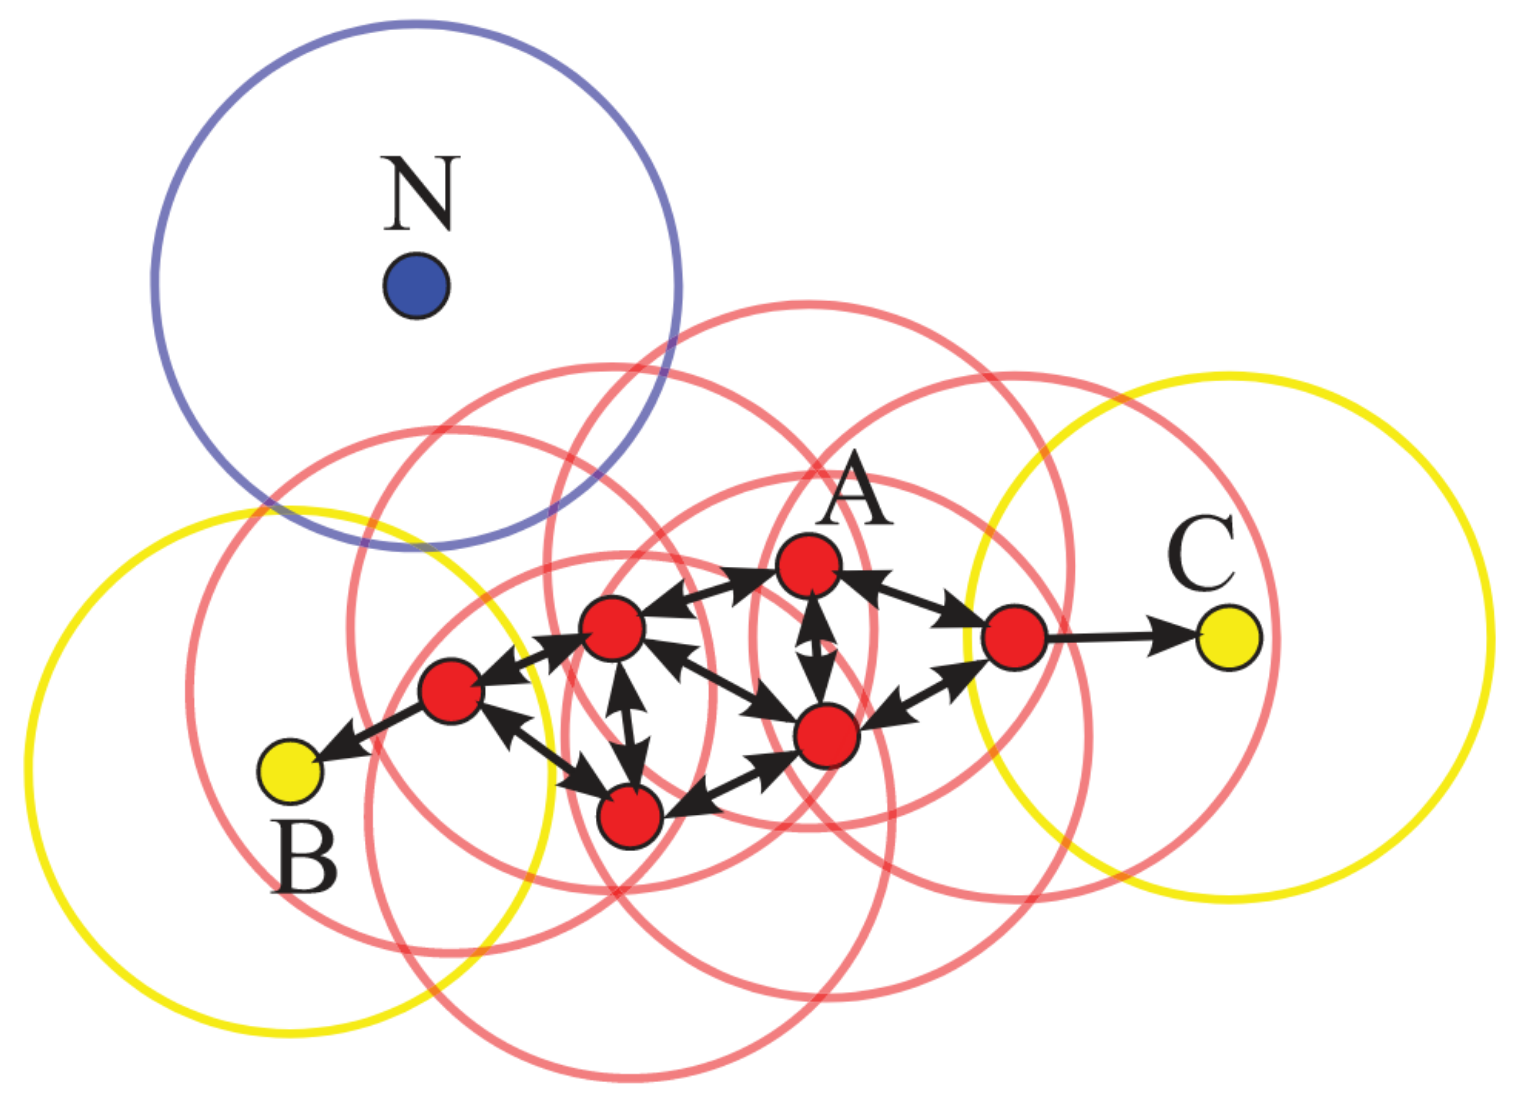
\includegraphics[width=0.5\linewidth]{obrazky-figures/dbscan}
		\caption{Illustration of DBSCAN cluster model}
		\label{dbscan_ilustration}
	\end{figure}

	Figure \ref{dbscan_ilustration} illustrates the model DBSCAN.
	In this illustration are defined parameters:
	\begin{itemize}
			\item minPts is 4
			\item $epsilon$ is indicated by circles
	\end{itemize}

	The abstracted algorithm is:
	\begin{enumerate}
			\item find neighbors in $\epsilon$ radius of every point, and find core points with more that minimum neigthnours (minPts)
			\item find connected core points on the graph and merge them into clusters.
			\item assign every non-core point to a core point if that non-core point is in $\epsilon$ radius of that core-point else assign it to noise.
	\end{enumerate}



	\begin{algorithm}[H]
		\SetKwData{syscall}{sc}
		\SetKwData{ids}{IDS}
		\SetKwData{argument}{arg}
		\SetKwData{level}{lvl}
		\SetKwData{numArgs}{num\_arg}
		\SetKwData{intervals}{intervals}
		\SetKwData{rules}{rules}

		\SetKwFunction{GetNumArgs}{get\_num\_args}
		\SetKwFunction{Append}{append}
		\SetKwFunction{getMinMax}{get\_minmax}

		\KwIn{intermediate data structure \ids}
		\KwOut{list of rules \rules}

		\caption{Smart optimization}\label{algo:weak}
		\ForEach{syscall \syscall in the \ids}{
			\ForEach{argument \argument in the syscall \syscall}{
				\numArgs $\leftarrow$ \GetNumArgs{p}\;
				\For{$\level \leftarrow 0$ \KwTo \numArgs}{
					\intervals.\Append{\getMinMax{\argument, \level}}\;
				}
				\rules.\Append{\syscall, \intervals}\;
			}
		}
	\end{algorithm}
\end{itemize}





\section{Parsing Expression Grammar}
Parsing expression grammar was introduced by Ford in 2004.
PEG is a type of analytic formal grammar which describes a formal language in terms of a set of rules for recognizing strings in the language.
This type of grammar is really similar to a top-down parsing languages.
As well it looks very similar to context-free grammars.

Parser that parses the PEG is named a packrat parser.
Packrat parser can be easily constructed for any language described by an LL($k$) or LR($k$) grammar, as well as for many languages that require unlimited lookahead and therefore are not LR.
Packrat parsers are also much simpler to construct than bottom-up LR parsers, making it practical to build them by hand.
It can directly and efficiently implement common disambiguation rules such as \textit{longest-match}, \textit{followed-by}, and \textit{not-followed-by}, which are difficult to express unambiguously in a context-free grammar or implement in conventional linear-time.
Finally, both lexical and hierarchical analysis can be seamlessly integrated into a single unified packrat parser.

The main disadvantage of packrat parsing is memory consumption.
The worst case asymptotic computational complexity is very similar to the conventional algorithms (linear in the size of the input).

The one of the many problems with right to left parsing algorithm is that it computes many results that are never needed.
Other inconvenience is that we must carefully determine the order in which the results for a particular column are computed.
\textit{Packrat parsing} is a lazy derivation of a tabular algorithm that solves both of these problems.
It computes results only when they are needed, in the same order as the original recursive descent parser would.
\cite{Ford:PEG}

\begin{table}[h]
	\begin{center}
  \begin{tabular}{lcl}
      Additive  & $\leftarrow$ & Multititve '+' Additive | Multitive \\
      Multitive & $\leftarrow$ & Primary '*' Multitive | Primary     \\
      Primary   & $\leftarrow$ & '(' Additive ')' | Decimal          \\
      Decimal   & $\leftarrow$ & '0' | \ldots | '9'
  \end{tabular}
  \end{center}
  \caption{Example of a grammar for a trivial language}
  \label{fig:pegtl:example}
\end{table}



% \section{Translator}
% This part is responsible for translation of IDS output to libseccomp.



\chapter{Development of strace2seccomp}
%code should be using libseccomp to be secure.
%test it with some fuzzer
\section{Logger}
There are many ways how can logger be implemented.
One of the first ideas were implement custom logger.
This idea wasn't bad but it will be a reinventing wheel.
Another way is using the logger implemented in boost library\footnote{http://www.boost.org/doc/libs/1\_63\_0/libs/log/doc/html/index.html}.
I decided to use this library because it was audited and tested by community, is widely supported and is well documented.

\section{Input}
As an input was used output from strace tool. As I mentioned earlier strace tool was
chosen because it is easy to use system call monitoring tool. It can monitor what observed
program demanded from kernel. With strace tool it is possible to trace child processes.
The main advantage of strace tool is that is doesn't need any of the source code files,
program has not to be compiled with extra flags or withount any library or
it does not have to be statically linked.

\subsection{Configure Strace to Produce Expected Input}
\label{sec:strace_config}

The output from strace tool has to be normalised before procesing with strace2seccomp.
The normalization is done by providing a few runtime arguments to strace tool.
Example:

\texttt{\$ strace -s 0 -xx -yy -o dataset -ff nautilus }
\\
I would like to describe what they are doing in the first place.\cite{strace_man}

\paragraph{-s} is a string size. We are setting a string size to zero because the
libseccomp does not have the ability to work with strings. It does not know how long is
the string or if it is really a string. By this option the filenames are not affected.
They are printed in full length.

\paragraph{-xx} this option will switch the format of strings to hexadecimal format.
It is much easier to parse strings in this format. It affects the filename as well.
This option is used because sometimes can occure a non ascii (UTF--8) character in filename.

\paragraph{-f} trace children processes.

\paragraph{-yy} will print protocol specific information associated with socket file descriptor.
It is here for future enhancements of strace2seccomp tool.

\paragraph{-o} is used for specifying the output file.

\paragraph{-ff} is helpfull when you are tracing a multiprocess program.
In this case it will create a multiple files in format
NAME.PID where NAME is a provided filename in option \texttt{-o} and PID is a process id.



\subsection{Strace grammar}
Strace produces structured output. Simplified version in extended Backus–Naur form (eBNF)\cite{ISO14977}
you can see in Figure \ref{strace_grammar_simple}.

\begin{figure}[h]
	\label{strace_grammar_simple}
	\begin{bnf*}
	\bnfprod{grammar}
		{\bnfpn{system\_call} \bnfor \bnfpn{signal} \bnfor \bnfpn{exit\_line}}\\
	\bnfprod{system\_call}
		{\bnfpn{sc\_name} \bnfsp  \bnfts{''(''} \bnfsp \{\bnfpn{argument}\} \bnfsp \bnfts{'')''} \bnfsp \bnfts{''=''} \bnfsp \bnfpn{digit}}\\
	\bnfprod{signal}
			{\bnfts{''+++ killed with''} \bnfsp \bnfpn{signal\_name} \bnfsp \bnfts{''+++''}}\\
	\bnfprod{exit\_line}
		{\bnfts{''+++ exited with''} \bnfsp \bnfpn{digit} \bnfsp \bnfts{''+++''}}\\
	\end{bnf*}
	\caption{Strace output grammar in eBNF}
\end{figure}

As you can see the grammar is composed of main parts that are \emph{system\_call}, \emph{signal} and \emph{exit\_line}.
For us are interesting the first one (\emph{system\_call}).
The system call is composed of a name of syscall, arguments and return code.
The argument can occur in a sequence and it is made of som atomic types
(value, constant, structure, array, string, address and there can be find comments as  well).
The string is in program represented as a place in memory but strace can dereference this address
and show it in analysis. This is the reason I mentioned it explicitly.


\section{Intermediate Representation}
How it looks and why?

\section{Output}
Chapter about creating output from IDS to libseccom or eBPF.
\subsection{libseccomp}
Something about using libseccomp.
\subsection{eBPF}
Maybe extension?
\subsection{C/C++ template}
Add it in appendix.
\subsection{Go template}
Add it in appendix.

\section{Heuristics and Optimizations}
Something about heuristics in global
\subsection{Minimax}
findin min and max for every arg. position.
\subsection{Strict}
input $\rightarrow$ output
\subsection{Smart}
we should use clustering \ldots
\subsubsection{Clustering}
What is clustering?
\subsubsection{Clustering algorithms used}
There are a lots of clustering algorithms. Find them \ldots.
\begin{itemize}
	\item{K-means}
	\item{DBSCAN\cite{Mahesh_Kumar2016}}
\end{itemize}



\chapter{Software Verification}
This chapter will describe activities used to assure quality control of the developed tool.
First, I want to introduce on which aspects we will focus.
One of the aspects is \textit{module testing}.
The main purpose of module testing is to detect errors in submodules, in communication among them, in passing data through data structures.
Another aspect of verification is \textit{system testing} merged with \textit{acceptance testing}.
In this type of testing we will check if the strace2seccomp tool has valid architectural design.
Next aspect which will be checked is \textit{static analysis}.
Static analysis is type of testing which does not requires run the program but requires a source code of the tool.
The static analyzer will analyse the source codes with different heuristics and produces a analysis of detected errors. % cite ITS lectures.



\section{Module Testing}
Module testing is part of whole quality control process.
This testing can provide us how functional are particular components and if they meet the requirements.
Table \ref{table:moduletesting} shows us the description of module's test suits.

\begin{table}[h]
	\centering
	\begin{tabular}{|l|p{10cm}|}
		\hline
		\textbf{Module / Component}	&	\textbf{Test descriptiom} \\ \hline
		Params 											& Validity of recognized runtime arguments \\ \hline
		StraceParser								& Syntax testing, validity of parsed data, correct error handling \\ \hline
	\end{tabular}
	\caption{Test plan}
	\label{table:moduletesting}
\end{table}

\subsection{Params Testing}
about using params class in custom test set and manualy check if the correct flags was ommited.

\subsection{StraceParser Testing}
StraceParser module is responsible for parsing the strace output and translates it to intermediate data structure.
Testing of this module can be done with various techniques.
First one which is used is fuzzy testing or fuzzing described in section above \ref{fuzzing}.
AFL fuzzer was used in the process.
\subsubsection{Fuzzing}
\label{fuzzing}
The term fuzzing was first used by professor Barton Miller who used fuzzing to test robustness of UNIX applications in 1989 \cite{Takanen:2008:FSS:1404500, Marhefka2013}.

\begin{itemize}
	\item{AFL} write sometihong about every fuzzer you mentioned
	\item{Bunny the Fuzzer}
	\item{Hongfuzz}
	\item{Radamsa}
	\item{oss-fuzz}
\end{itemize}
\subsubsection{Fuzzing results}
Show some results from afl.
\subsubsection{Grammar testing}
If you got time write grammar tester. or find one .. dunno

\subsection{Algorithms}
How should we test if algorithms?
\subsection{Optimizer}
how should we test this adapter?
\subsection{Output}
Testing correctness of a Output generator
\begin{itemize}
	\item{C/C++}
	\item{Go}
\end{itemize}

\section{System and Acceptance Testing}
\subsection{Testing on real app}
\subsection{USBGuard}

\section{Static analysis}
Any bugs?

\section{Test Requirements}

\section{Results}
Which bugs have you found.



%=========================================================================
